%% The following is a directive for TeXShop to indicate the main file
%%!TEX root = diss.tex

\chapter{A Description of 3D Reconstruction}
\label{ch:3DRecon_Desc}
In Chapter~\ref{ch:3DRecon_Taxo}, we introduce a taxonomy of 3D reconstruction which maps algorithms to the problem space according to visual/geometric characteristics of the object. However, without a formal `language', \ie a model and representations, this mapping would be largely empirical. Expressing the conditions within which an algorithm works well without a formal definition of the problem space prevents formulating a well defined problem.

In this chapter, we attempt to extend this taxonomy by providing a description of the 3D reconstruction problem which allows for a well defined specification of the conditions surrounding the problem. This description abstracts away from the functional specification of \textit{how} to estimate a reconstruction. We first propose a formal definition of the 3D reconstruction problem in Section~\ref{sec:3DRecon_Def}. Next, section~\ref{sec:3DRecon_Model} proposes a model to 3D reconstruction by selecting various key \textit{aspects} of the problem space that are crucial for describing the appearance of the object. Section~\ref{sec:3DRecon_Rep} outlines concrete representations of the proposed model. Section~\ref{sec:3DRecon_Exp} provides examples of expressing common 3D reconstruction problems using the proposed model and representations. These following four layers represent the description of our accessible 3D reconstruction framework: Definition, Representation, Model, and Expression.

% Computer vision problems require, among other factors, a model of the problem domain~\cite{little1985phdthesis} and appropriate representations. The model characterizes the relevant properties of the elements in the domain and analyze their relations. The representations describe an object's properties selected by the model to facilitate a solution of the problem.

\section{Definition}
\label{sec:3DRecon_Def}
We will first provide definitions of some basic concepts, which include general computer vision concepts such as scene, camera, and image. We then define a few other terms that are closely related to the reconstruction problem. We then provide reasonable approximations for a more practical definition of the problem as a whole.

\subsection{Basic notations}
We will use the following notations: $\{C_n\}_{n=0}^{N-1}$ represents the camera set, which includes both intrinsic and extrinsic parameters; $\{I_n\}_{n=0}^{N-1}$ represents the set of all images; $\{L_n\}_{n=0}^{N-1}$ represents the set of light sources.

\noindent\textbf{Definition 1 (Scene)} The scene $S$ is the four-dimensional joint spatio-temporal target of interest.

\noindent\textbf{Definition 2 (Image)} The image refers to the 2D observation of the 3D scene $S$ on the image plane of camera $C_i$ at time $t_0$, which is modelled as: $I_i = T(S, C_i, L_0, t_0)$, or on the image plane of $C_0$  under the light source $L_i$ at time $t_i$, $I_i= T(S, C_0, L_i, t_i)$, where $T$ is the geometric/radiometric transformation.

$T$ can be a geometric transformation which determines the 2D coordinates of a 3D point, or a radiometric transformation which determines the intensity/irradiance information from the information of illumination, viewing direction and surface orientation.

\subsection{Segment and Scell}
\noindent\textbf{Definition 3 (Segment)} A segment ($seg$) is a distinct region in the image, and is the most basic element in the image, which can be considered as a generalized pixel. 

For instance, a segment can be a pixel, a window area, an edge, a contour, or a region of arbitrary size and shape.

\noindent\textbf{Definition 4 (Cue)} Cues are the visual or geometric characteristics of the segments $seg$ that can be used for reconstruction, denoted as $cue(seg)$.

For instance, the cue can be the texture within a window area, the intensity/colour value of a pixel, or the object contour, etc.

\noindent\textbf{Definition 5 (Scell)} A scell (scene element, denoted as $sc$) is a volume in the scene which corresponds to at least one segment. A scell can be considered as a generalization of a voxel.
 % However, a scell is not necessarily distinct since

\noindent\textbf{Definition 6 (Property)} Properties are the visual and geometric characteristics of the scell $sc$, which would influence the cues of a segment, denoted as $prop(sc)$.

The property of the scell can be the 3D position or orientation information, visual texture, reflectance, surface orientation, roughness, convacity, etc.

The relation between the terms defined above is shown in Figure~\ref{fig:scell_seg}.
\begin{figure}[!htbp]
\centering
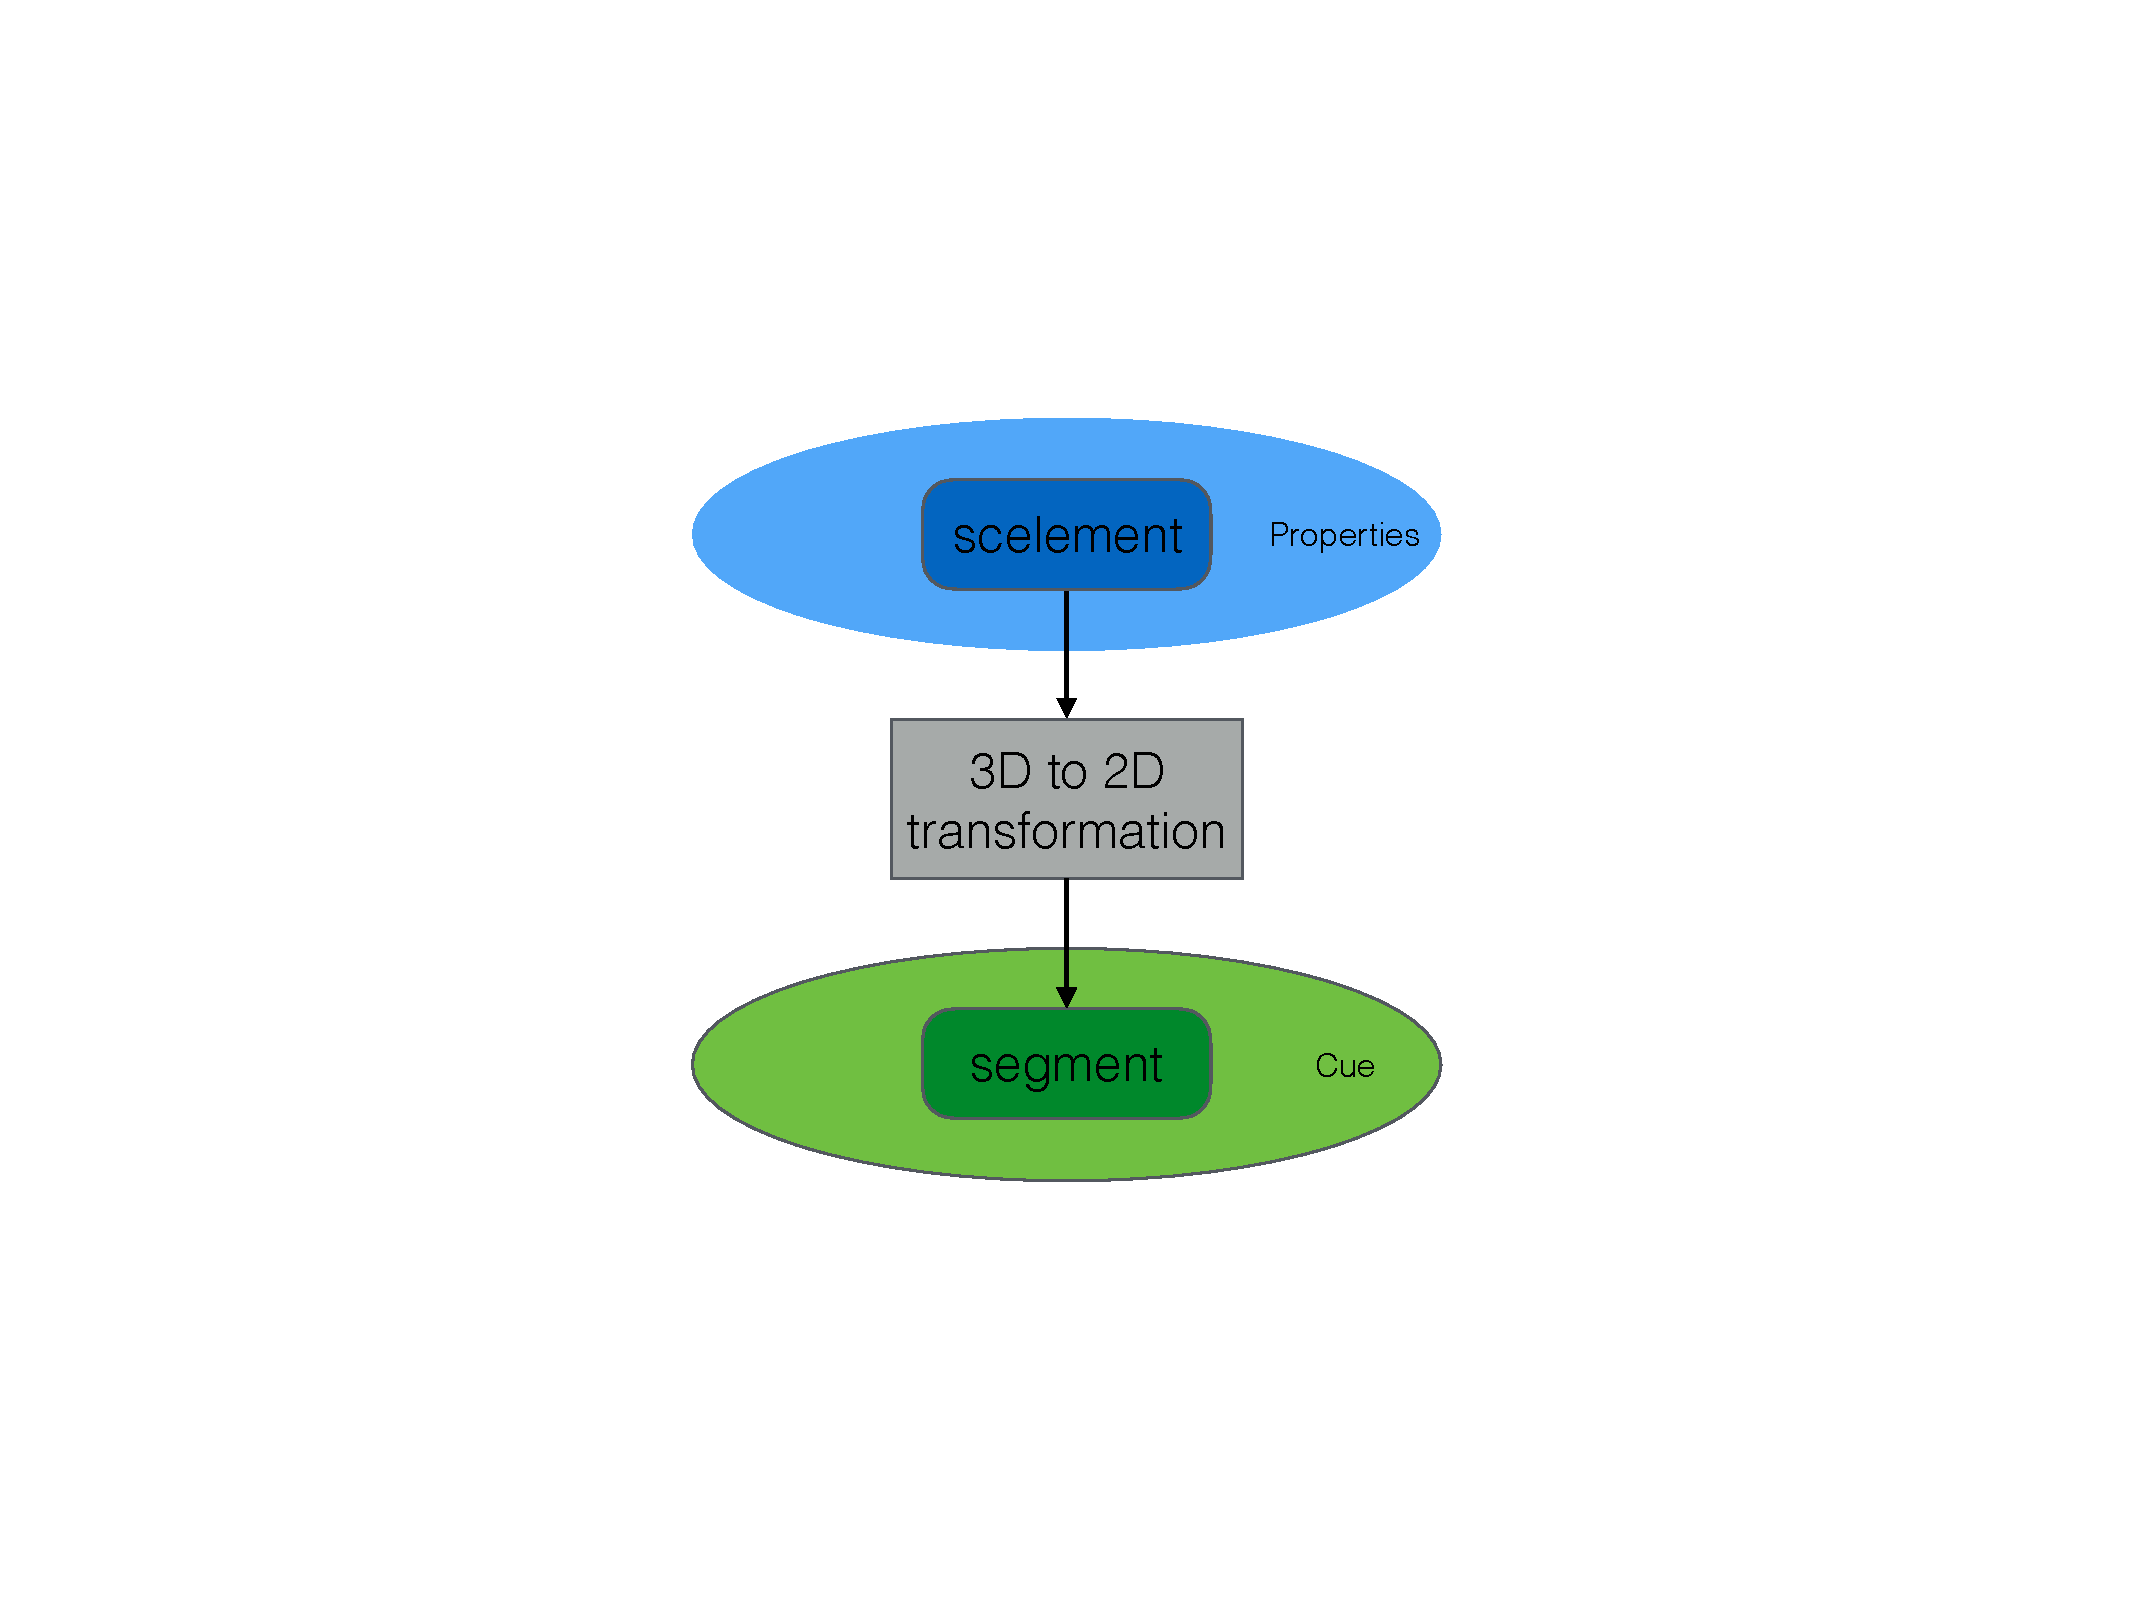
\includegraphics[width=0.5\textwidth]{model/seg_scell}
\caption{Relation between a scell and a segment}
\label{fig:scell_seg}
\end{figure}

% \textbf{Definition (Representation)} The scell can be represented as a voxel, a depth value, a 3D point/patch, or a surface normal, etc, which is denoted as $rep(sc)$.

\subsection{Consistency}
Every photograph of a 3D scene taken from a camera $C_i$ partitions the set of all possible scenes into two families, those that reproduce the photograph and those that do not. We characterize this constraint for a given shape and a given radiance assignment by the notion of \textit{consistency}.

\noindent\textbf{Definition 7 (Consistency criterion)} The consistency criterion checks whether the properties of a scell $sc$ can produce the cues observed in the corresponding segment $seg$.
\begin{align*}
consist(prop(sc), cue(seg)) = 1 &\Rightarrow \textit{consistent}\\
consist(prop(sc), cue(seg)) = 0 &\Rightarrow \textit{not consistent}
\end{align*}

\noindent\textbf{Definition 8 (Segment consistency)} Let $S$ be the scene. A scell $s\in S$ that is visible from $C_i$ is consistent with the image $I_i$ if and only if the consistency criterion is true.

\noindent\textbf{Definition 9 (Image consistency)} A scene $S$ is image consistent with image $I_i$ if any scell $\forall s\in S$ visible from the camera $C_i$ is segment consistent with this image.

\noindent\textbf{Definition 10 (Scene consistency)} A scene $S$ is scene consistent with a set of images $\{I_n\}_{n=0}^{N-1}$ if it's image consistency with each image $I_i\in \{I_n\}_{n=0}^{N-1}$ in the set.

\subsection{Formal Definition}
\noindent\textbf{Definition 11 (3D reconstruction problem)} Given a set of images $\{I_n\}_{n=0}^{N-1}$ captured by cameras $\{C_n\}_{n=0}^{N-1}$, or under a set of light sources $\{L_n\}_{n=0}^{N-1}$, find a set of scells $\{sc_m\}_{m=0}^{M-1}$ such that any scell is consistent with the visible images in the set $\{I_n\}_{n=0}^{N-1}$, \ie $\forall sc_i\in \{sc_m\}_{m=0}^{M-1}$, we the have following:
\begin{align*}
consist(prop(sc_i), cue(seg_{(i, j)})) = 1.
\end{align*}
where $seg_{(i, j)}$ is the corresponding segment of $sc_i$ in camera $C_j$. Alternatively, 3D reconstruction tries to find a set of scells $\{sc_m\}_{m=0}^{M-1}$ that are scene consistent with the image set $\{I_n\}_{n=0}^{N-1}$

\subsection{Applied Definition}
While the definition presented above gives a formal definition of the problem of 3D reconstruction, it is not necessarily applicable in a practical setting. In this section, we extend this formal definition to an approximate, yet applied version.

\noindent\textbf{Definition 12 (Consistency score)} The consistency score measures the similarity betweem a scell $sc$ and the corresponding segment $seg$.
\begin{align*}
consist(prop(sc), cue(seg)) &= x \text{, } x\in[0, 1]\\
consist(prop(sc), cue(seg)) &= 1 \Rightarrow \textit{consistent}\\
consist(prop(sc), cue(seg)) &= 0 \Rightarrow \textit{not consistent}
\end{align*}

\noindent\textbf{Definition 13 (Applied consistency criterion)} A scell $sc$ and a segment $seg$ are considered consistent if the the consistency score is above a pre-defined threshold $\epsilon$.
$$
consist(prop(sc), cue(seg)) > \epsilon
$$

% \noindent\textbf{Some more definitions} $\sum_{n\in I'}consist(prop(sc_i), cue(seg_{(i, n)}))$

\noindent\textbf{Definition 14 (Applied 3D Reconstruction Problem)} Given a set of images $\{I_n\}_{n=0}^{N-1}$ captured by cameras $\{C_n\}_{n=0}^{N-1}$, or under a set of light sources $\{L_n\}_{n=0}^{N-1}$, find a set of scells $\{sc_m\}_{m=0}^{M-1}$ such that the consistency score between the set of scells and their corresponding segments $\{seg_{(i, j)}\}_{i=0,j=0}^{M-1,N-1}$ are maximized.
$$
\mbox{maximize} \quad \sum_{j=0}^{N-1}\sum_{i=0}^{M-1} consist(prop(sc_i), cue(seg_{(i, j)}))
$$

\section{Model}
\label{sec:3DRecon_Model}
Models and representations are fundamental for vision problem solving. Models select characteristic properties of an object, and representation describes the model selected object properties to facilitate a solution of a class of problem. A model facilitates the representation of aspects in reality that are useful in a particular problem domain~\cite{bolles19863dpo}. For instance, surface orientation is one component of the surface geometry model, and the corresponding representation can be surface normal or curvature. Another example is colour, which is a component of a material model, and where RGB space is the corresponding representation of the colour.

We select the subset of properties used for object taxonomy in Chapter~\ref{ch:3DRecon_Taxo} as the main components of our model. The model consisting of these key properties is shown in Table~\ref{tab:3DRecon_model}.
\begin{table}[h]
  \centering
  \begin{tabular}{l|*{5}{c}}
  \hline
  \textbf{Property} & Texture & Lightness & Reflectance & Roughness & Concavity\\
  \hline
  \end{tabular}
  \caption{Model of the 3D reconstruction problem. Properties are selected from the taxonomy in Chapter~\ref{ch:3DRecon_Taxo}.}
  \label{tab:3DRecon_model}
\end{table}

% In addition to these properties, there are requirements that can be imposed to the final reconstruction result. These requirements include but not exclude:

% \begin{table}[h]
%   \centering
%   \begin{tabular}{l|*{5}{c}}
%   \hline
%   \textbf{Requirement} & Accuracy-first & Completeness-first & Orientation-first & Roughness & Concavity\\
%   \hline
%   \end{tabular}
%   \caption{Model of the 3D reconstruction problem: requirements}
%   \label{tab:3DRecon_model}
% \end{table}

\section{Representation}
\label{sec:3DRecon_Rep}
Based on the proposed definition and model of the 3D reconstruction problem, we need to further define our representations so that the 3D reconstruction problem can be expressed using our proposed model. We need to turn our attention to how to represent the properties used in the proposed model.

% We look at the \textit{cues} that are utilized by 3D reconstruction techniques and their corresponding contributing properties. In Chapter~\ref{ch:3DRecon_Taxo}, we explored a new taxonomy of 3D reconstruction based visual/geometric cues. Now we need to investigate the visual and geometric properties of the object that can affect those cues. This section is organized by the visual/geomtric cues, and the visual/geomtric properties are investigated in each section.

% \subsection{Segment and scell}
% As defined in section~\ref{sec:3DRecon_Def}, a segment is the 3D to 2D transformation of a scell. Here we discuss concrete examples of segment and scell.

% \subsubsection{Pixel and voxel}
% In the image plane, a pixel is a square of size $1\times 1$. In the matrix representation of an image $I$, a pixel is an entry of the matrix, $I(x, y)$. A voxel is a 3D regular cube, and the center of which is projected to the center of the pixel.
% \begin{figure}[h]
% \centering
% 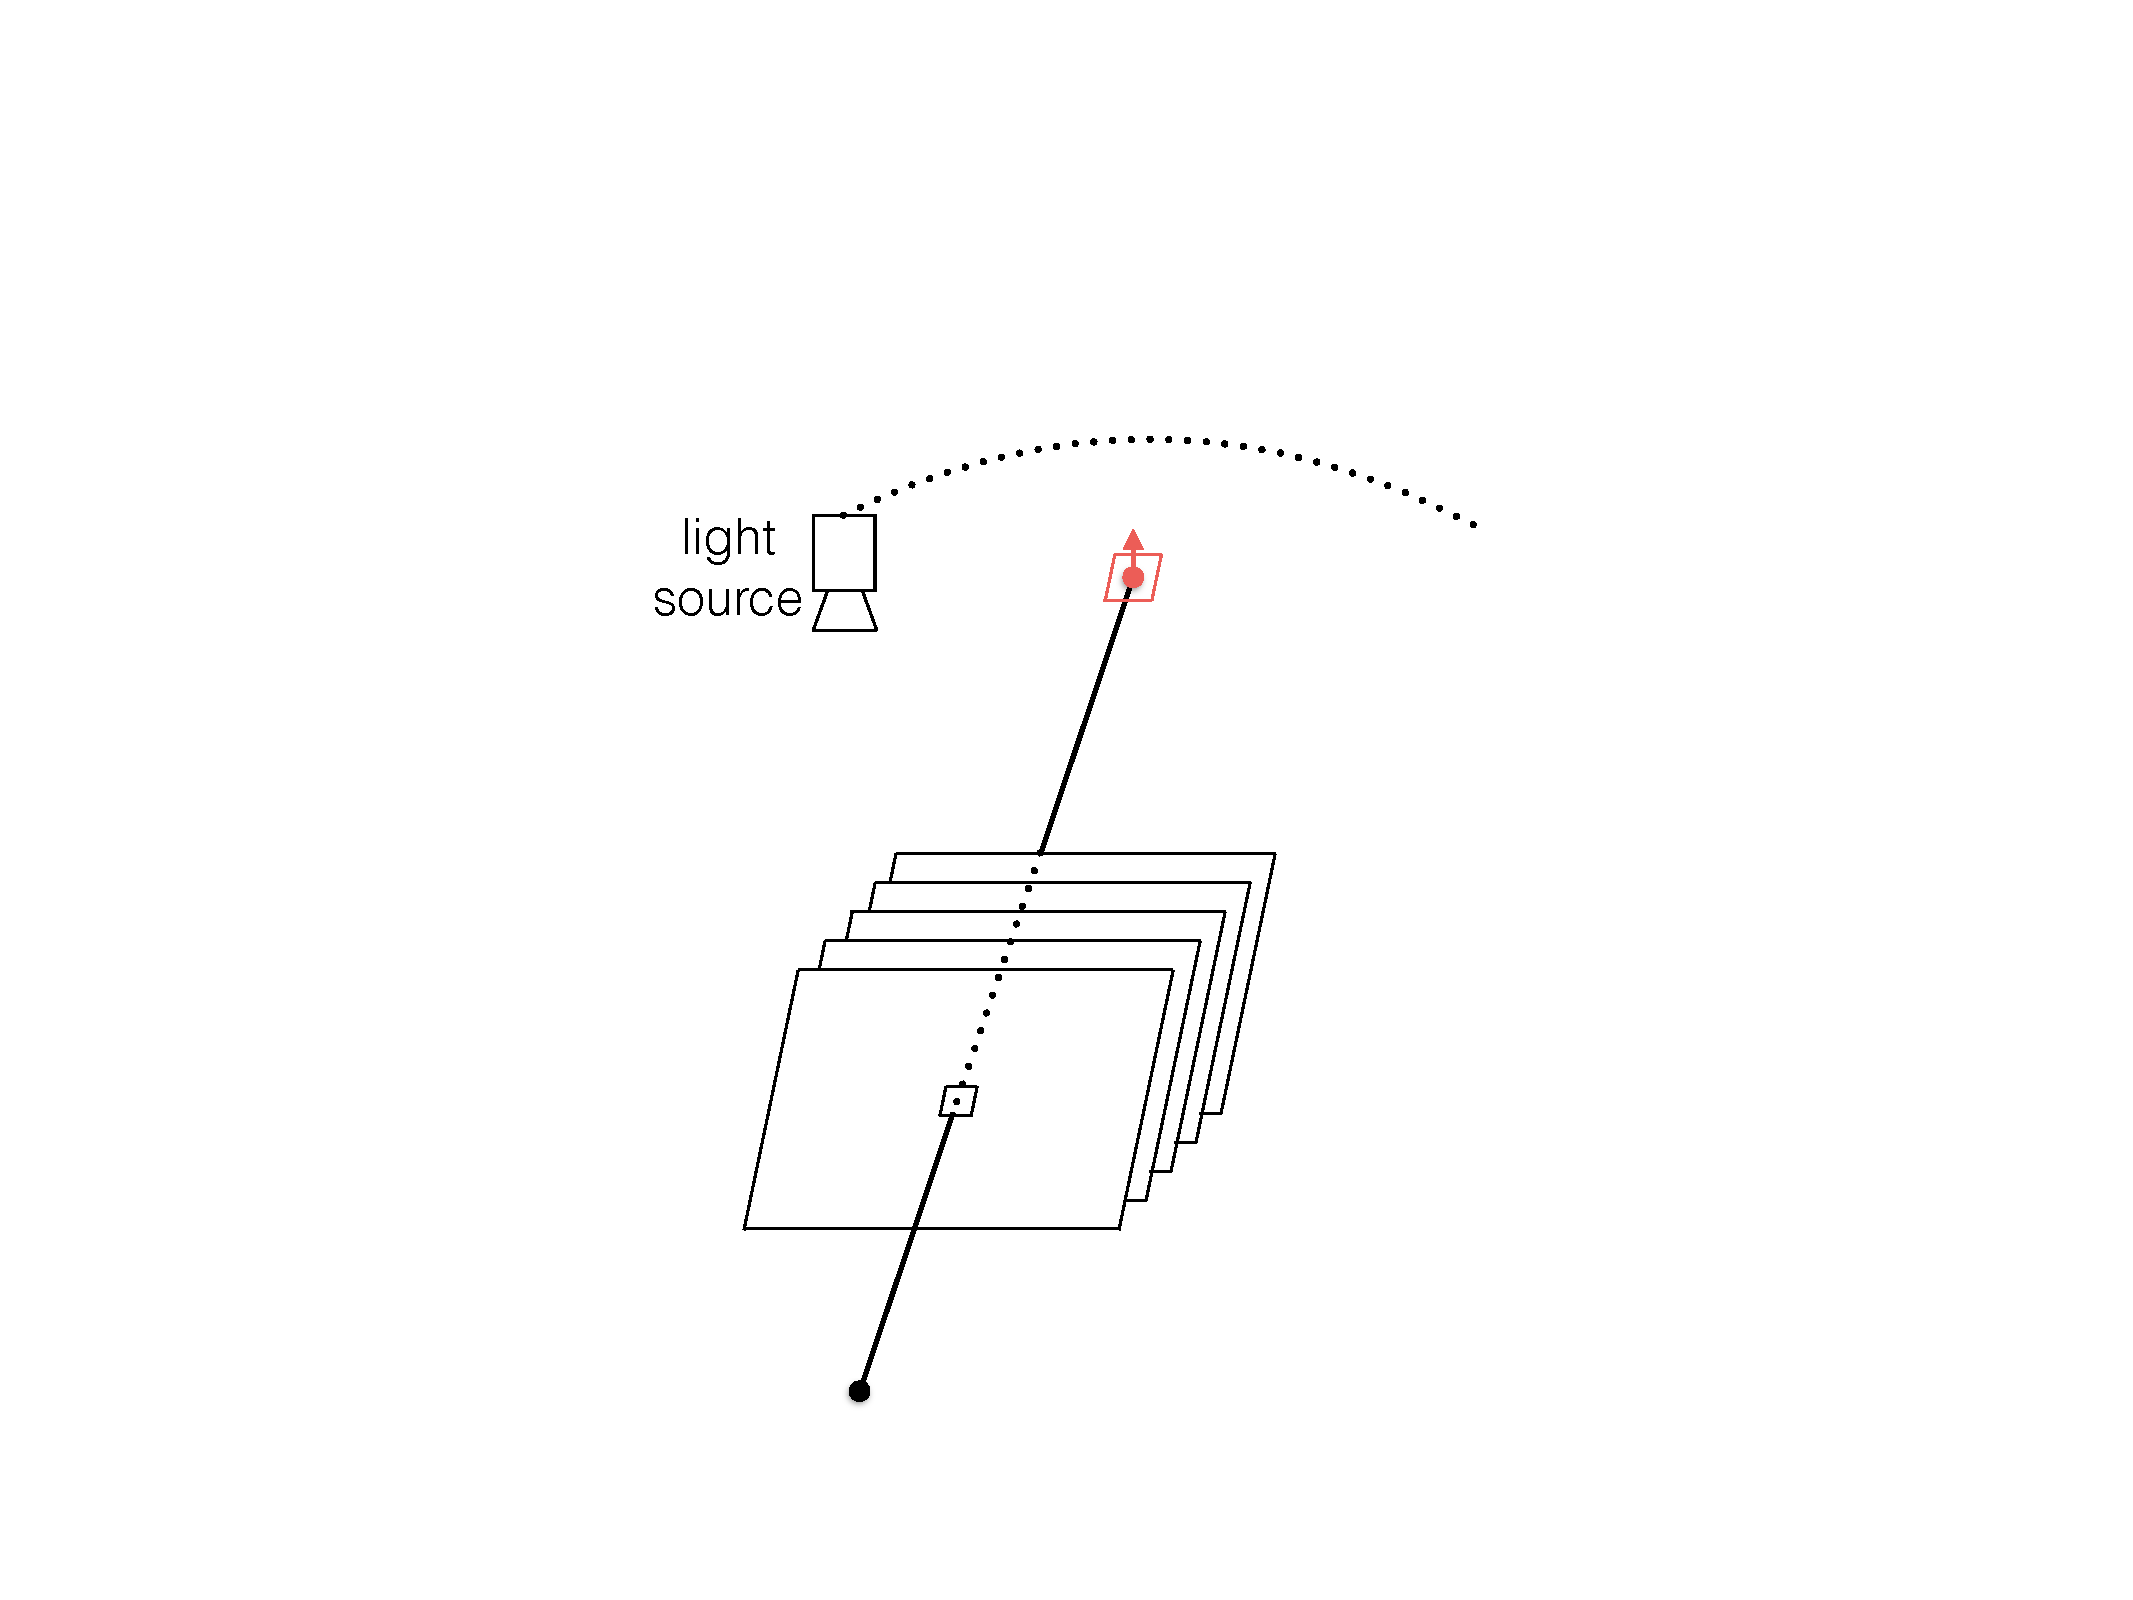
\includegraphics[width=0.5\texturewidth]{model/pixel_voxel}
% \caption{Pixel and voxel}
% \end{figure}

% \subsubsection{Silhouette and bounding edge}


% \subsubsection{Window area and patch}
% A window area is contained in a $w\times w$ regular square, and the surface patch is a 3D point of $p\times p$ with a normal vector.
% \begin{figure}[h]
% \centering
% 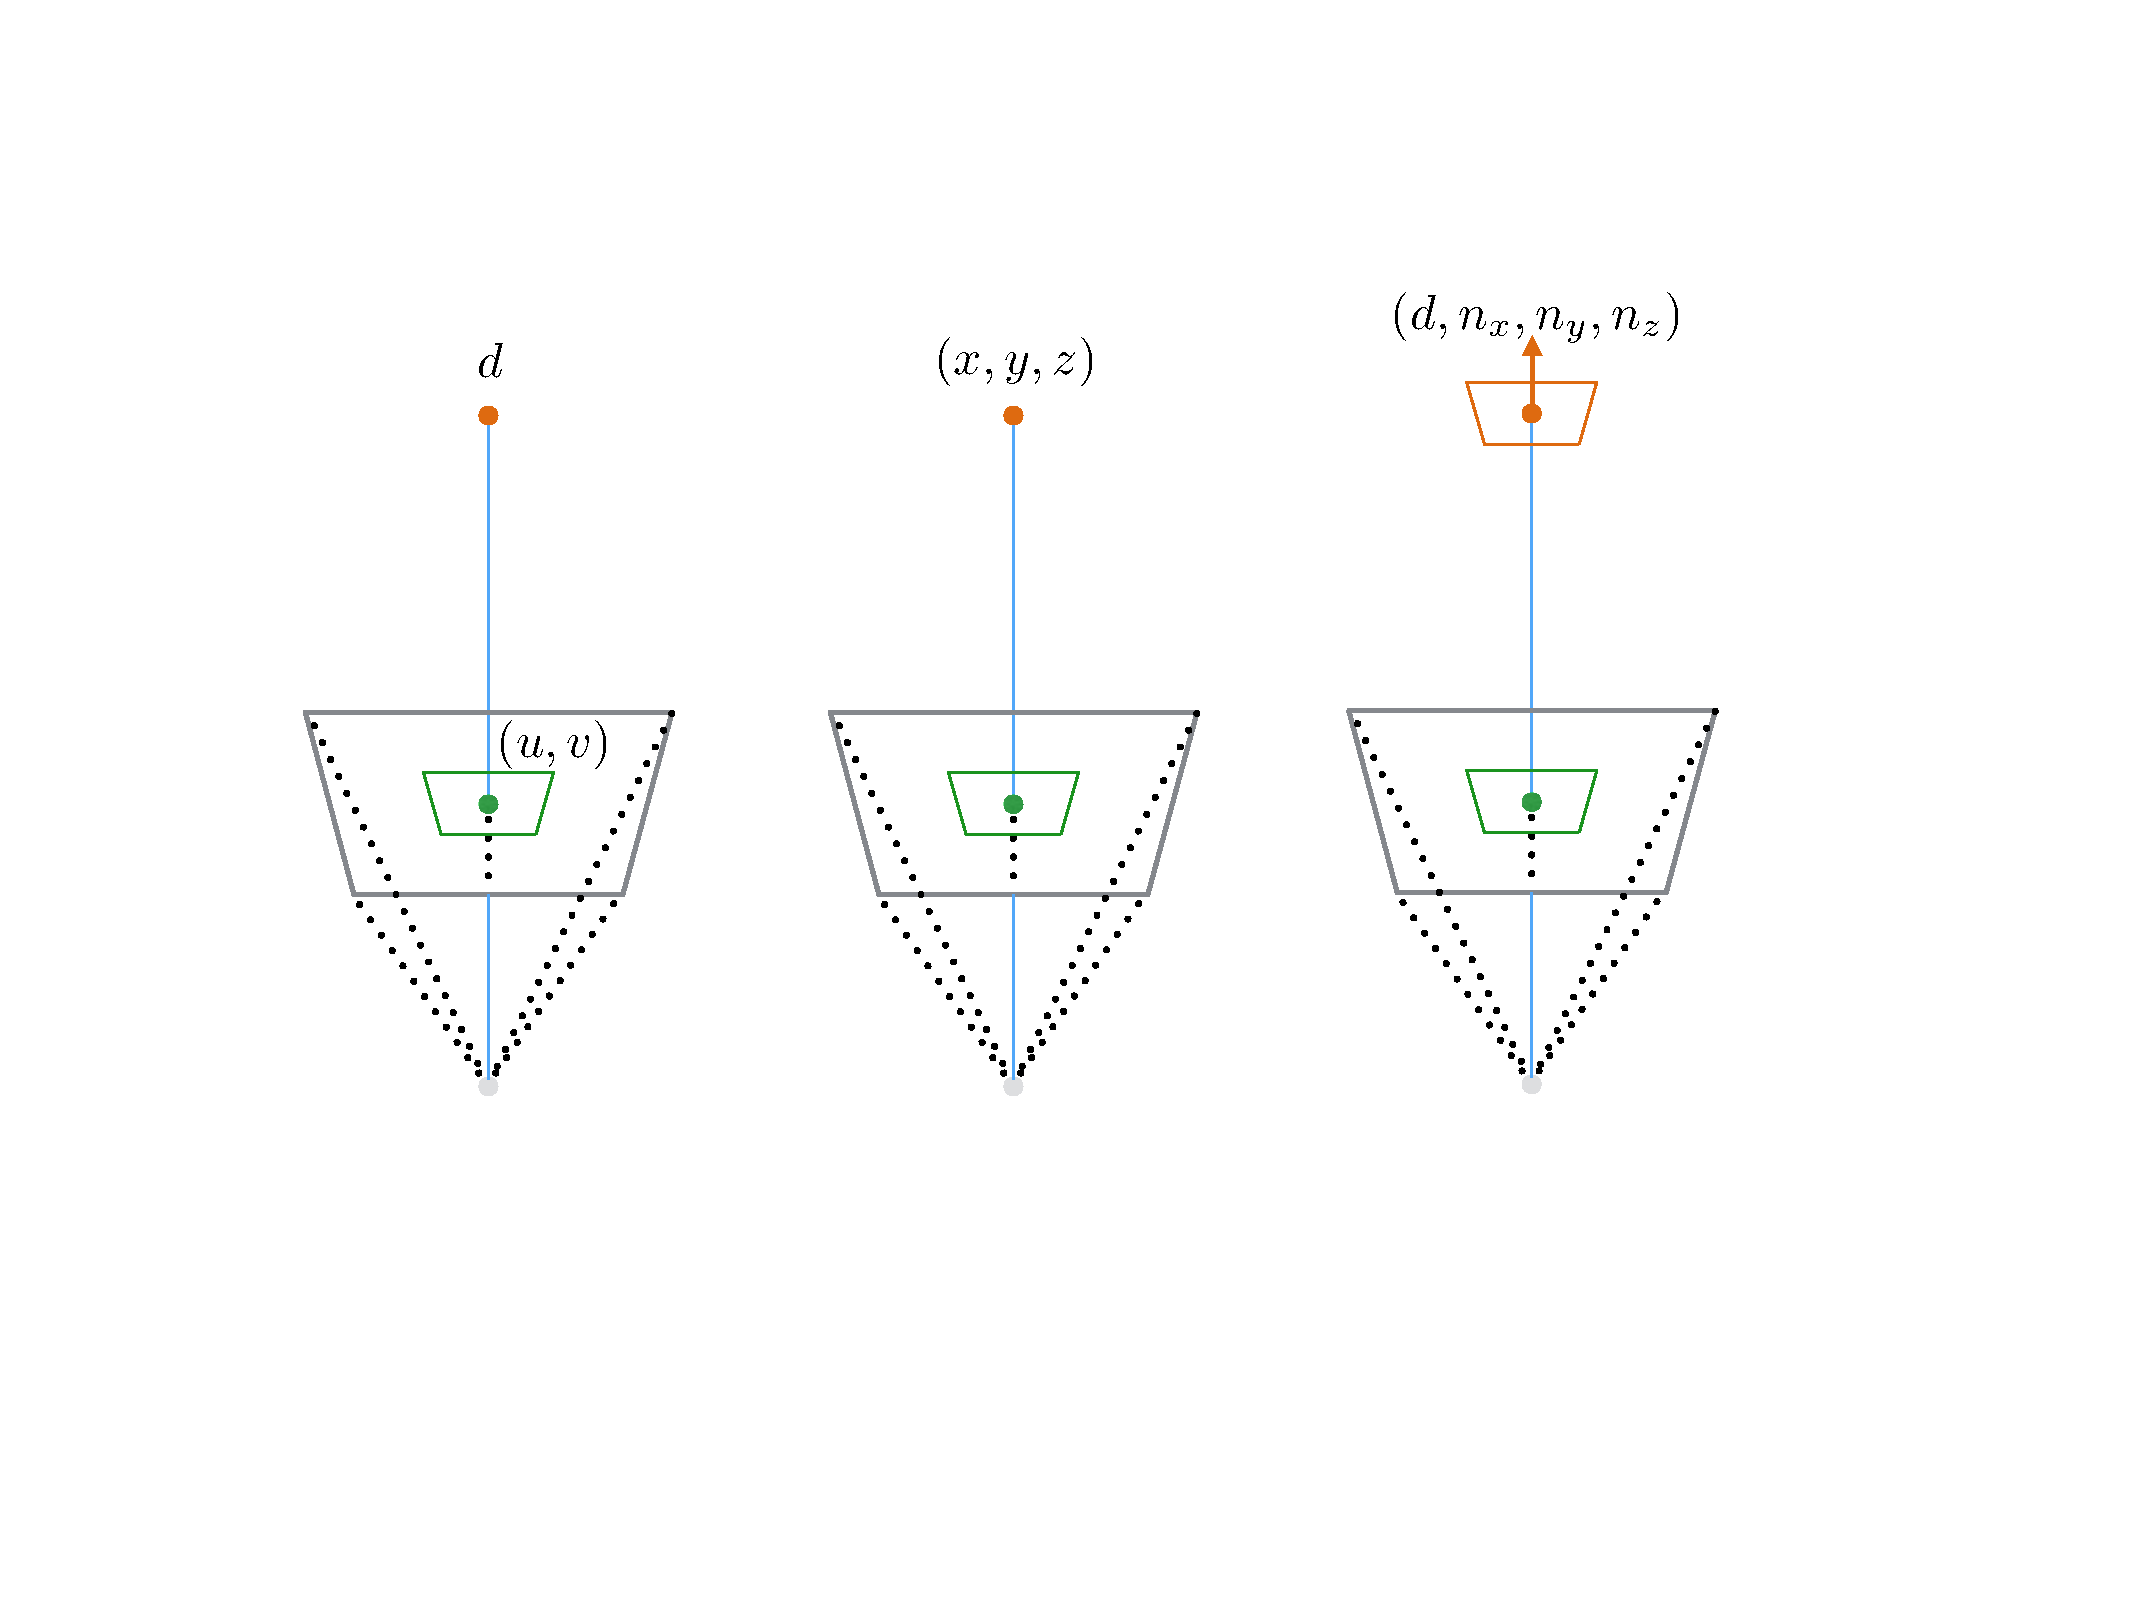
\includegraphics[width=0.8\textwidth]{model/window_patch}
% \caption{a window area and a surface patch}
% \end{figure}

% \subsection{Cues and properties}
% As defined in Chapter~\ref{sec:3DRecon_Def}, cue is the characteristics of the segment while property is that of the scell. For each cue observed in a segment, we discuss the underlying properties that have an impact on it.

\subsection{Texture}
Texture is one of the most important cues for many computer vision algorithms. It is generally divided into two categories, namely \textit{tactile} and \textit{visual} textures. Tactile textures refer to the immediate tangible feel of a surface, whereas visual textures refer to the visual impression that textures produce to the human observer, which are related to local spatial variations of simple stimuli like colour, orientation and intensity in an image. Here we focus only on visual textures, as they are more widely used in the stereo vision research. The term `texture' hereafter refers exclusively to `visual texture' unless mentioned otherwise.

Although texture is an important component in computer vision, there is no precise definition for the notion of texture itself. The main reason for this is that natural textures often exhibit separate yet contradicting properties, such as regularity versus randomness, or uniformity versus distortion, which can hardly be described in a unified manner. 
% Haralick considers a texture as an ``organized area phenomenon'' which can be decomposed into `primitives' having specific spatial distributions~\cite{haralick1979statistical}. This definition, also known as structural approach, comes directly from human visual experience of texture. These primitives are organized in a particular spatial structure indicating certain underlying placement rules. Alternatively, as Cross and Jain suggested, a texture is ``a stochastic, possibly periodic, two-dimensional image field''~\cite{cross1983markov}, which is also known as \textit{stochastic approach}.

% For s regular textures, there are two basic dimensions on which it may be described. The first dimension is for describing the primitives out of which the texture is composed, and the second dimension is for the description of the spatial dependence or interaction between the primitives of an image texture. The first property is concerned with tonal primitives and local properties, and the second dimension is concerned with the spatial organization of the tonal primitives.

There are various properties that make texture distinguishable: scale/size/granularity, orientation, homogeneity, randomness, etc. However, due to the diverse and complexe nature of textures, it is a challenging task to generate a synthetic texture solely from these semantic properties, or the other way around, derive parameters from a given texture. The stereo vision community often takes a simplified approach, classifying textures into two categories, regular and stochastic, by degree of randomness. A regular texture is formed by regular tiling of easily identifiable elements (texels) organized into strong periodic patterns. A stochastic texture exhibits less noticeable elements and displays rather random patterns. Most of the real world textures are mixtures of these two categories. In this thesis, we adopt this simplification and consider \textit{texture randomness}, which is the amount of distortion in the texture. Thus, a uniform texture has low \textit{texture randomness} whereas a highly textured surface has \textit{texture randomness}.

% Most texture synthetic research has focused on data-driven or statistical approaches. For the data-driven approach, the generated texture is not general enough whereas it's not intuitive enough for the statistical approach. Thus we turn to an approach that is more tailored to the stereo vision problem. Based on the observations from practical tests, stereo algorithms work well under the condition of non-uniform texture, even for textures caused by shadow. This is theoretically plausible as stereo vision tries to find the correspondence based on the `distinctiveness' of the texture. Therefore, as long as the surface is covered by distinct texture, it doesn't matter what the basic texture element is. Thus the most significant attributes of the texture is coverage, \ie the percent of the surface that is covered, and it's the focus of this thesis.

% Texture is formally defined as a set of texture element or \textit{texels} occuring in some regular, or repeated, or random pattern. Texture gives us information about the \textit{spatial arrangement} of the colours or intensities in an image. However, it is something that is easy to recognize, but hard to define. 

% Here we only consider visual textures, which is the result of shape and reflection. Therefore, a surface with varying reflectance property can produces a textured surface, a flat surface with fixed reflectance property under different illuminations can also achieve textured effect. Even very weak texture can be a strong cue to object reconstruction as manifested by the Middlebury `Dino' dataset.

\subsection{Lightness}
When light strikes a surface, it may be reflected, transmitted, absorbed, or scattered; usually, a combination of these effects occurs. The intensity/colour information received by a sensor is thus determined, among other factors, by the amount of light available after these interactions. Here, we consider intensity as caused solely by reflection, since this is one of most common phenomena experienced and is the easiest to analyze. Generally, we assume that all effects are local, thus global effects such as interreflection and transmission, among others, are omitted. This is called a \textbf{local interaction model}. 
% Lightness ranges from `black' to `white' in the grey scale axis, and colour is a superset of intensity, which takes into account the spectral composition of light. Both lightness and colour depend on illumination, surface normal, surface reflectance, and viewing direction.

In order to understand the contributing factors of pixel intensity/colour, we need an in-depth understanding of reflection, \ie how light is reflected off of a surface patch, and the relation between material and intensity values. The radiometric formation of an image consists of three separate processes, \textit{light-matter interaction}, \textit{light-lens interaction}, and \textit{light-sensor interaction}.

\subsubsection{Definition of Radiometric Terms}
Below is a list of radiometry terms, see Figure~\ref{fig:radiometry_terms} for an illustration:
\begin{itemize}
\item Solid angle ($d\omega$): 3D counterpart of angle, $d\omega=\frac{dA \cos\theta_i}{R^2}\mathit{ (steradian)}$.
\item Projected solid angle ($d\Omega$): $d\Omega = \cos\theta d\omega$.
\item Incident radiance ($\mathbf{L_i(\theta_i, \phi_i)}$): light flux received from the direction $(\theta_i, \phi_i)$ on a unit surface area, unit $\mathit{ (watt\cdot m^{-2}\cdot steradian^{-1})}$.
\item Irradiance ($\mathbf{E_i(\theta_i, \phi_i)}$): light Flux (power) incident per unit surface area from all direction, $\mathbf{E_i(\theta_i, \phi_i)}=\int_{\Omega_i} L_i(\theta_i, \phi_i) d\Omega_i \mathit{ (watt/m^2)}$.
\item Surface radiance ($\mathbf{L_r(\theta_r, \phi_r)}$): light flux emmited from a unit surface area in the direction $(\theta_r, \phi_r)$, unit $\mathit{ (watt\cdot m^{-2}\cdot steradian^{-1})}$.
\end{itemize}

\begin{figure}[!htbp]
\centering
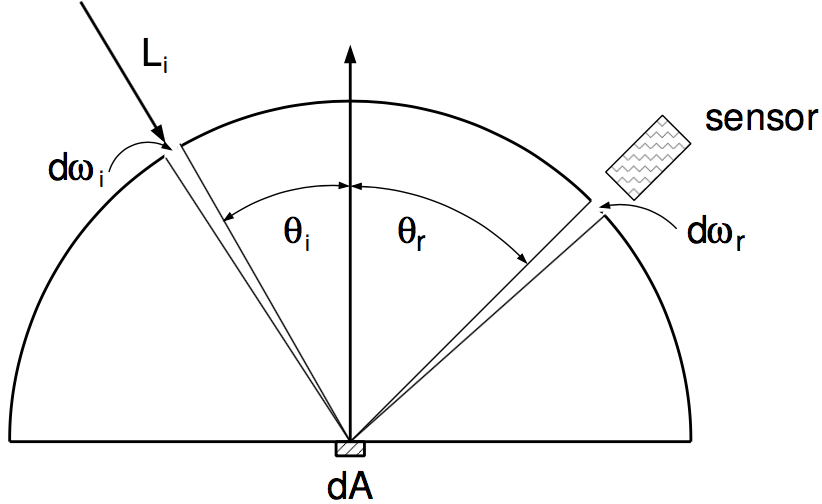
\includegraphics[width=0.5\textwidth]{model/radiometry_terms.png}
\caption{Illustration of light-matter interaction.}
\label{fig:radiometry_terms}
\end{figure}

\subsubsection{Light-matter interaction}
The relation between the incoming illumination and reflected light is modelled using the \textit{bidirectional reflectance distribution function} (BRDF). The BRDF is defined as

\noindent\textbf{Definition (BRDF)} the ratio of the surface radiance $\mathbf{L_r(\theta_r, \phi_r)}$ to the irradiance $\mathbf{E_i(\theta_i, \phi_i)}$, \ie $f(\theta_i, \phi_i, \theta_r, \phi_r)=\frac{E^{surface}(\theta_i, \phi_i)}{L^{surface}(\theta_r, \phi_r)}$.
\begin{figure}[!htbp]
\centering
\begin{tikzpicture}[node distance=2cm, auto]
\node (light_rad) [data] {Incident Radiance};
\node (material) [model, right of=light_rad, xshift=2cm] {Material};
\node (scene_rad) [data, right of=material, xshift=2cm] {Scene Radiance};
\draw [arrow] (light_rad) -- (material);
\draw [arrow] (material) -- (scene_rad);
\end{tikzpicture}
\caption{The light-matter interaction.}
\label{fig:light_matter_interact}
\end{figure}

\textit{Diffuse albedo} or surface albedo is the proportion of incident light that is reflected by the surface. 
% It should be noted that albedo is not an intrinsic property of a surface. Instead, for any surface, the albedo depends on the spectral and angular distributions of the incident light.

\subsubsection{Light lens interaction}
The assumption made in vision is that radiance is constant as it propagates along a ray. Therefore, the scene radiance is the same as the radiance passing through the lens. It can be further shown that the image irradiance received by the sensor is proportional to the scene radiance, thus the relation between \textit{scene radiance} and \textit{image irradiance} is linear.
\begin{figure}[!ht]
\centering
\begin{tikzpicture}[node distance=2cm, auto]
\node (scene_rad) [data] {Scene Radiance};
\node (lens) [model, right of=scene_rad, xshift=2cm] {Lens};
\node (irradiance) [data, right of=lens, xshift=2cm] {Image Irradiance};
\draw [arrow] (scene_rad) -- (lens);
\draw [arrow] (lens) -- (irradiance);
\end{tikzpicture}
\caption{The light-lens interaction.}
\label{fig:light_lens_interact}
\end{figure}

\subsubsection{Light sensor interaction}
The camera response function relating image irradiance at the image plane to measured pixel intensity values is a non-linear mapping. A linear relation can be retrieved by radiometric calibration.
\begin{figure}[!ht]
\centering
\begin{tikzpicture}[node distance=2cm, auto]
\node (irradiance) [data] {Image Irradiance};
\node (sensor) [model, right of=irradiance, xshift=2cm] {Sensor};
\node (intensity) [data, right of=sensor, xshift=2cm] {Intensity};
\draw [arrow] (irradiance) -- (sensor);
\draw [arrow] (sensor) -- (intensity);
\end{tikzpicture}
\caption{The light-sensor interaction.}
\label{fig:light_sensor_interact}
\end{figure}

In conclusion, as long as the \textit{light-sensor interaction} is considered as a linear mapping (as most vision algorithms do) or calibrated in a pre-processing step, the pixel intensity value is linearly related to surface reflectance, which is characterized by BRDF. There are 4 DoF in spatially-invariant BRDF, and for a simplified case - Lambertian reflectance, the BRDF is degenerated to \textit{diffuse albedo}, which is the representation we adopt for the property of intensity.

% The reflectance of light also depends on the incident direction. Specifically, light that lands on a surface at a grazing angle will be much more likely to reflect, see Figure~\ref{fig:alb_ang}. We take into account the Fresnel effect in the synthetic stage, thus we consider the albedo with small incident angle.
% \begin{figure}[h]
% \centering
% 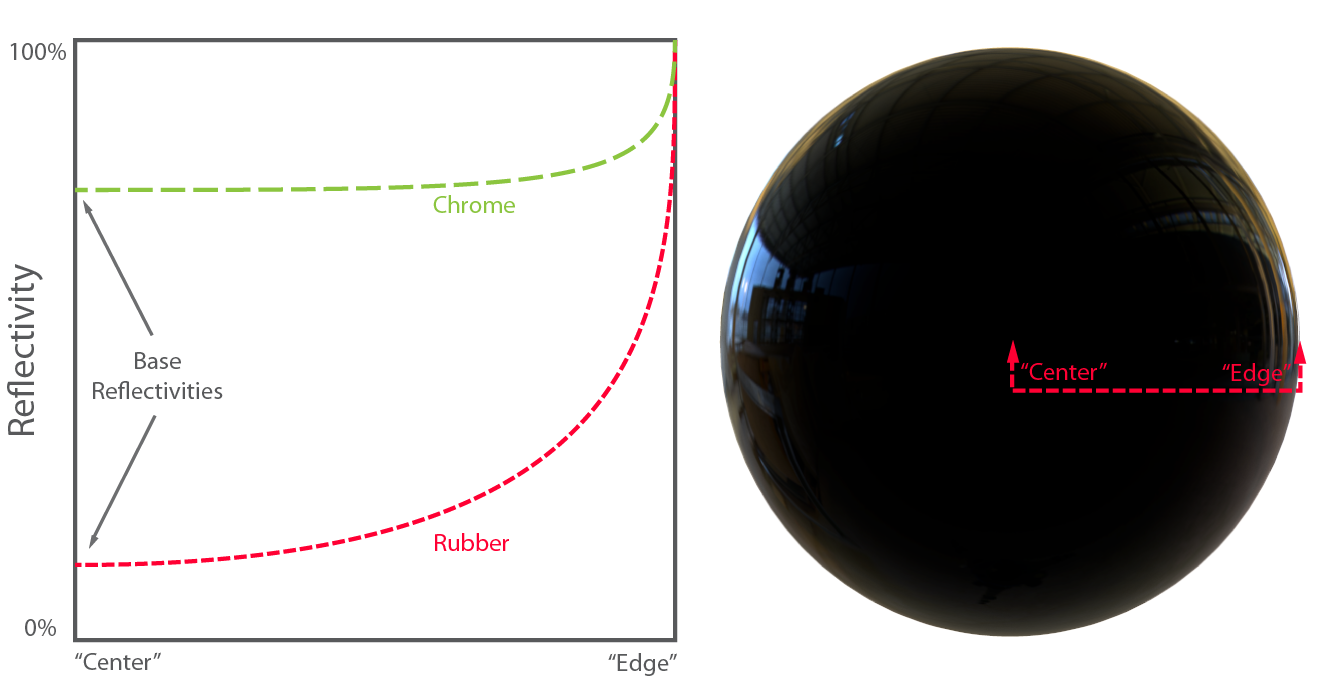
\includegraphics[width=0.5\textwidth]{model/reflectance_angle}
% \label{fig:alb_ang}
% % \caption{Spectral reflectance curves for aluminium (Al), silver (Ag), and gold (Au) metal mirrors at normal incidence.}
% \end{figure}

\subsection{Specularity}
Specular surfaces reflect light in nearly a single direction when the microscopic surface irregularities are small compared to light wavelength, and no subsurface scattering is present~\cite{nayar1989surface}. Unlike diffuse reflections, where we experience the lightness and colour of an object, specular reflections carry information about the structure, intensity, and spectral content of the illumination field. In other words, specular reflection is simply an image of the environment, or the illumination field, distorted by the geometry of the reflecting surface. In Figure~\ref{fig:spec_ref}, the image no longer reflects the original colour of the surface, which is red. Instead it shows a distorted image of the environment. A purely specular surface is a mirror, which is rare in nature. Most natural materials exhibit a mixture of specular and diffuse reflections. Variations in microscopic surface geometry can cause specular reflections to be scattered, blurring the image of the environment in an amount proportional to surface roughness. We use a numeric \textit{specular} value to denote the proportion of a material's specularity, with 0 being completely diffuse, and 1 being completely specular (mirror like).
\begin{figure}[!htbp]
\centering
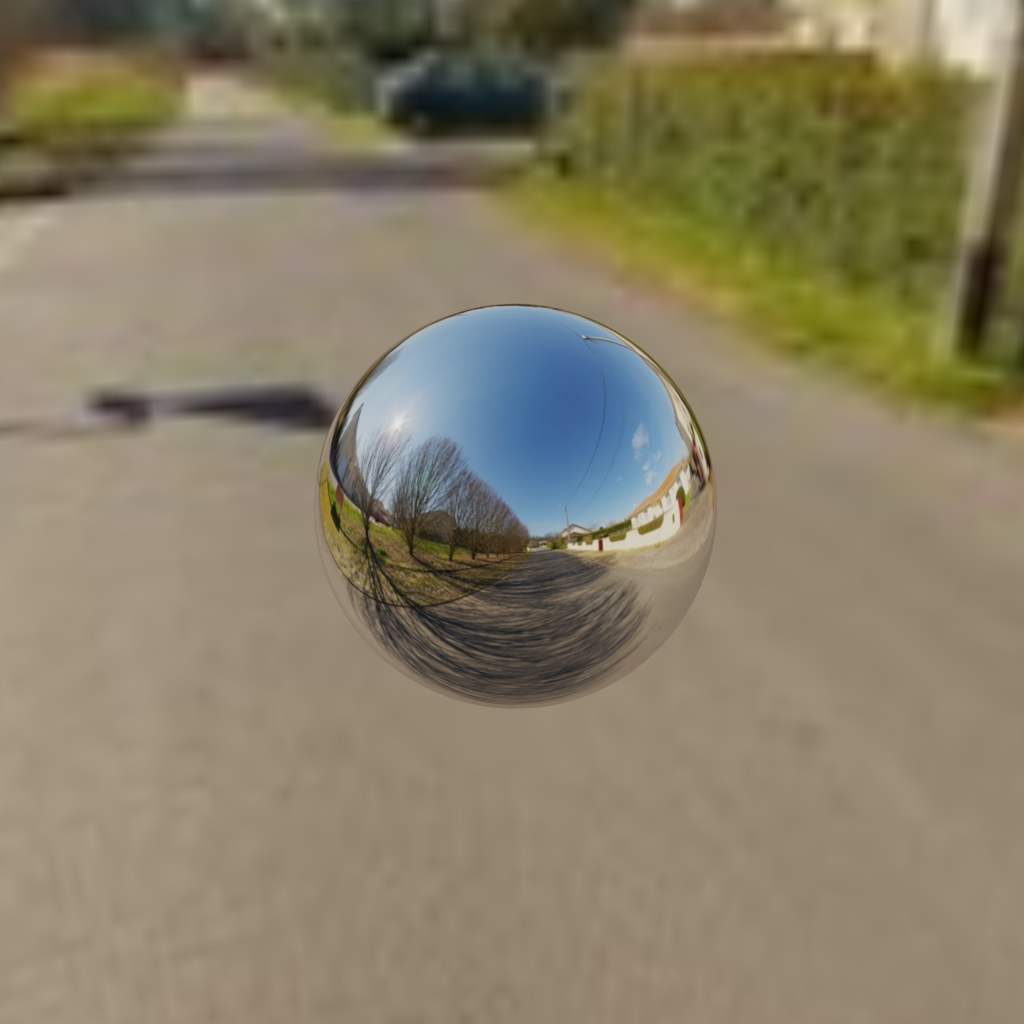
\includegraphics[width=0.3\textwidth]{model/spec_ref}
\caption{A \textbf{red} specular sphere. The surface reflects light in a mirror-like way, showing a distorted environment. Since no diffuse reflection exists, the colour of the surface is no longer visible.}
\label{fig:spec_ref}
\end{figure}

\subsection{Roughness}
Roughness, which refers to the microscopic shape characteristics of a surface, contributes to the way in which light is reflected off of a surface. A smooth surface may reflect incident light in a single direction, while a rough surface may scatter the light in various directions. We need prior knowledge of the microscopic surface irregularities, or a model of the surface itself, to determine the reflection of incident light.

Possible surface models are divided into 2 categories: surfaces with exact known profiles and surfaces with random irregularities. An exact profile may be determined by measuring the height at each point on the surface by means of a sensor such as the stylus profilometer. This method tends to be cumbersome and impractical, hence, it is more reasonable to model the surface as a random process, where it is described by a statistical distribution of either its height above a certain mean level, or its slope with respect to its mean (macroscopic) slope. We will use the second statistical approach in this section.

% \textit{Height Distribution Model} The height coordinate of the surface is expressed as random function of the coordinates $x$ and $y$.
% \begin{figure}[h]
% \centering
% \includegraphics[width=0.5\textwidth]{model/surface_representation_1}
% \caption{Surface height distribution model}
% \end{figure}

% The shape of the surface is determined by the probability distribution of $h$. For instance, let $h$ be normally distributed, with mean value $\bar{h}=0$ and standard deviation $\sigma_h$. Then, the distribution of $h$ is given by:
% $$
% p_h(h)=\frac{1}{\sqrt{2\pi}\sigma_h}e^{-\frac{h^2}{2\sigma_h^2}}
% $$

% The $\sigma_h$ is the root-mean-square of $h$ and represents the roughness of the surface. The surface is not uniquely described by the distribution of $h$, as it does not tell us anything about the distance between the hills and valleys of the surface.

% The surfaces below have the same height distribution function, i.e., the same mean value and standard deviation. However, they don't resemble each other in appearance.
% \begin{figure}[h]
% \centering
% \includegraphics[width=8cm]{model/same_mean_sd}
% \caption{Surface height distribution model}
% \end{figure}

% An autocorrelation coefficient $C(\tau)$ is introduced, that determines the correlation (or lack of independence) between the random values assumed by the height $h$ at two surface points $(x_1, y_1)$ and $(x_2, y_2)$, separated by a distance $\tau$. The autocorrelation coefficient can be:
% $$
% C(\tau)=e^{-\frac{\tau^2}{T^2}}
% $$

% where $T$ is the *correlation distance*. Therefore, the above surfaces have small and large correlation distances respectively.

% \subsubsection{Slope Distribution Model}
% We can think of a surface as a collection of planar micro-facets. A large set of micro-facets constitutes an infinitesimal surface patch that has a mean surface orientation $\vec{n}$. Each micro-facet has its own orientation, which may deviate from the mean surface orientation by an angle $\alpha$.
% \begin{figure}[h]
% \centering
% 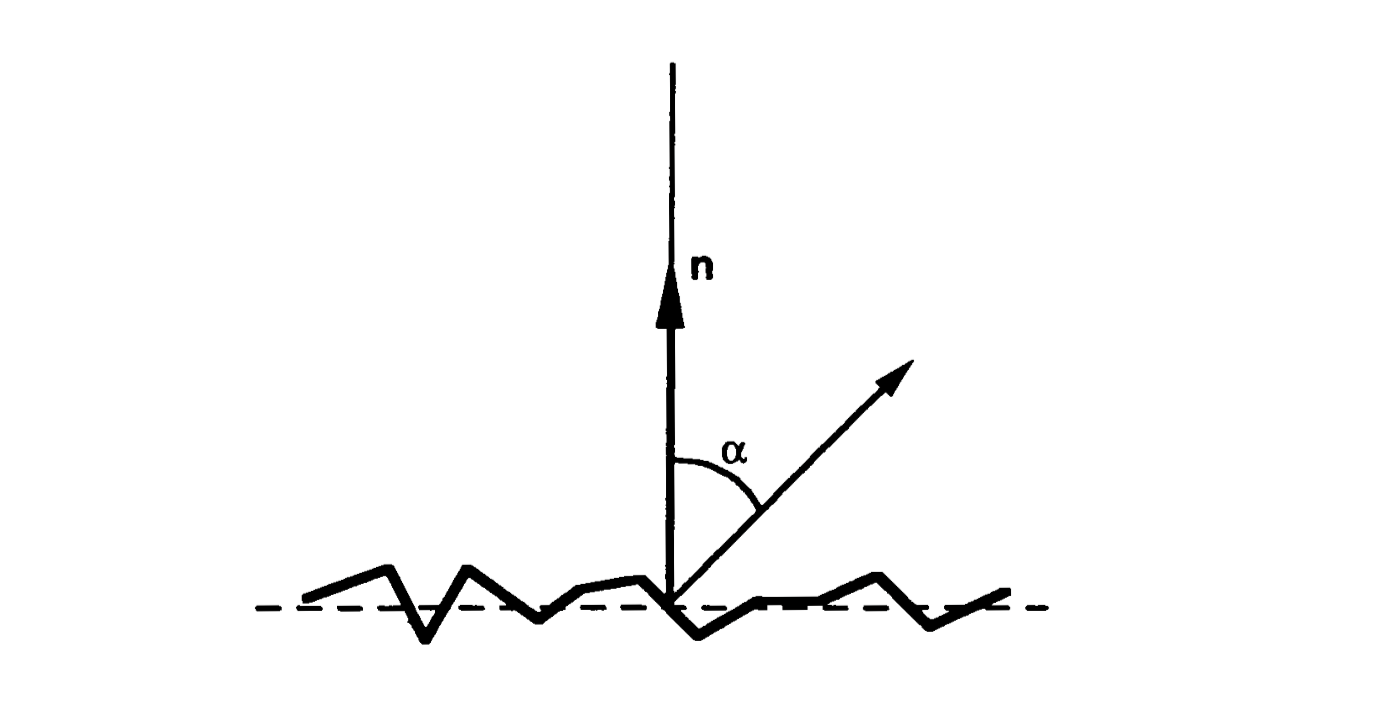
\includegraphics[width=0.7\textwidth]{model/surface_representation_2}
% \caption{Surface Slope Distribution Model}
% \end{figure}

% We will use the parameter $\alpha$ to represent the slope of individual facets. Surfaces can be modeled by a statistical distribution of the micro-facet slopes. If the surface is isotropic, the probability distribution of the micro-facet slopes can be assumed as rotationally symmetric w.r.t the mean surface normal $\vec{n}$.  Therefore, facet slopes can be described by a one-dimensional probability distribution function. For instance, the surface may be modeled by assuming a normal distribution for the facet slope $\alpha$, with mean value $\bar{\alpha}=0$ and standard deviation $\sigma_\alpha$, where the larger $\sigma_\alpha$ can be used to model rougher surfaces:
% $$
% p_\alpha(\alpha)=\frac{1}{\sqrt{2\pi}\sigma_\alpha}e^{-\frac{\alpha^2}{2\sigma_\alpha^2}}
% $$

% The surface model is determined by a single parameter $\sigma_\alpha$ While autocorrelation coefficient is important, the concept of slope correlation is more difficult to interpret and is not that useful in the generation of surface, which results in a weaker model compared to the height model. However, slope distribution model is popular in the analysis of surface reflection, as the scattering of light rays is dependent on the local slope of the surface and not the local height of the surface.

% surface roughness will affect the fresnel and specularity

\subsection{Concavity}
Concavity can cause self-shadow or interreflection effects, which can severely impede the accuracy of active methods. Since concavity is invisible in the silhouette images, methods that utilize silhouette information may also fail to reconstruct concavities. Concavity can be measured by \textit{surface curvature}, which is defined as the inverse of the radius of a tangentially intersecting circle/sphere. We include concavity in our model for the sake of completeness. However, we decide to omit this property since concavity will introduce global light transport including cast shadow and interreflection, and so on, which violates our assumption of a \textbf{local interaction model}.

% \subsubsection{Silhouette}
% \textbf{Concavity} is not shown in the silhouette image, thus methods that utilize silhouette information may fail to reconstruct concavities. Concavity is measured by \textit{surface curvature}.

\section{Expression}
\label{sec:3DRecon_Exp}
Now that we have a proposed model and representation of 3D reconstruction problem, we can express the six proposed object classes using this description. The expression of the reconstruction problem is shown in table~\ref{tab:express}.
\begin{table}[!htbp]
  \centering
  \begin{tabular}{l*{5}{c}}
  \hline
  \textbf{Class \#} & Texture randomness & Albedo & Specularity & Roughness & Concavity\\
  \hline
  Class 1 & 0.2 & 0.8 & 0.2 & 0.8 & 0.2\\
  Class 2 & 0.2 & 0.8 & 0.5 & 0.2 & 0.2\\
  Class 3 & 0.8 & 0.8 & 0.2 & 0.8 & 0.2\\
  Class 4 & 0.8 & 0.2 & 0.2 & 0.8 & 0.2\\
  Class 5 & 0.8 & 0.8 & 0.5 & 0.2 & 0.2\\
  Class 6 & 0.8 & 0.2 & 0.5 & 0.2 & 0.2\\
  \hline
  \end{tabular}
  \caption{Expression of 3D reconstruction problem for the object classss proposed in Chapter~\ref{ch:3DRecon_Taxo}.}
  \label{tab:express}
\end{table}